\documentclass[class=report, crop=false]{standalone}
\usepackage{amsmath}
\usepackage{mathtools}
\usepackage{algorithm}
\usepackage{algorithmic}
\usepackage{graphicx}
\usepackage{hyperref}
\usepackage[utf8]{inputenc}
% make sure to keep these two lines the very last in the preamble
% if you want to add packages add them before not after these two lines
\usepackage[subpreambles=true]{standalone}
\usepackage{import}
\begin{document}

Dans ce chapitre,nous allons présenter la conception détaillée des méthodes exactes sur lesquelles notre choix d'implementation s'est porté:

\begin{enumerate}

\item Le branch and bound

\item Une version améliorée du branch and bound

\item La recherche exhaustive

\item La programmation dynamique
\end{enumerate}
Dans le but de montrer l’applicabilité de ces méthodes, comparer leurs performances et montrer leurs limites, nous effectuerons des tests empiriques et comparatifs sur des benchmarks d’un coté, et sur des instances générées par notre propre générateur d’instances d’un autre coté.
\section{Branch and bound}
\begin{itemize}
    \item L'algorithme Branch-and-Bound (B \&B) que nous avons implémenté tente de ranger un objet à la fois en fonction de l’ordre initial des objets. 
    \item Au niveau j de l’arbre, B \&B crée un noeuds fils pour chaque boite ouverte et range l’objet j dans cette boîte si c’est possible. il crée aussi un noeuds supplémentaire qui représente l’ouverture d’une nouvelle boîte, et il range l’objet j dans cette boîte.
    \item En pratique, au niveau 1 de l’arbre l’objet 1 est rangé dans la boîte 1 , au niveau 2 l’objet 2 est rangé dans la boîte 1 ou dans une nouvelle boîte 2 ,...etc 
    \item A chaque noeud, on résout un sous problème de taille (n-k) du bin packing, où les k premiers objets ont déjà été emballés.
    \item L’opération du rangement d’un objet i au niveau k consiste à permuter entre les éléments list(K) et list(i). On va avoir comme sortie une liste d’objets ordonnées selon l’ordre de rangement, il suffit ensuite de remplir les boîtes par les objets dans leur nouvel ordre pour générer la solution (l’emplacement de chaque objet dans les boîtes) 
\end{itemize}

\begin{figure}[h]
    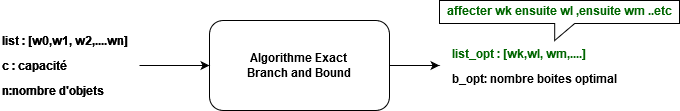
\includegraphics[width=\linewidth]{../figures/diagr1.png}
\end{figure}
\subsection{Pseudo-Code}
% \begin{algorithm}
%    \caption{Bin packing}   
%\end{algorithm}
\subsubsection*{Evaluation d'un noeud (Borne L1)}
L’évaluation d’un nœud est calculée en sommant 2 parties, le nombre de boîtes déjà utilisées bcount et une estimation du nombre de boîtes qu’on va ouvrir encore pour contenir les objets restants. Cette estimation est obtenue en divisant la somme des poids restants sumwt sur la capacité d’une boîte. On soustrait de la somme des poids restants, l’espace vide 
restant dans la dernière boîte ouverte, car ce dernier peut contenir des objets. On obtient ainsi la formule suivante :  

\begin{figure}[h!]
    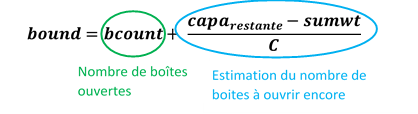
\includegraphics[width=8cm]{../figures/formule1.png}
\end{figure}
\paragraph{exemple 1: }
List= {10,50,25,80,70,75,35,70} ;   C = 100 
\begin{figure}[h!]
    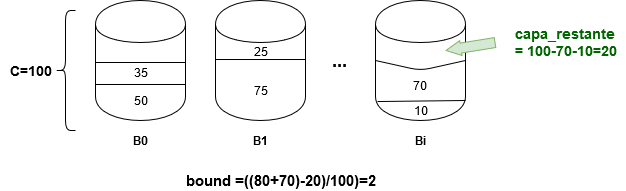
\includegraphics[width=10cm]{../figures/example1.png}
\end{figure}
\paragraph{exemple 2: }
n= 5 ; $W_{j}$={49,41,34,33,29} ; c=100 
on pose : $b_j$= le numéro de boîte qui contient l’objet j.

\begin{figure}[h!]
    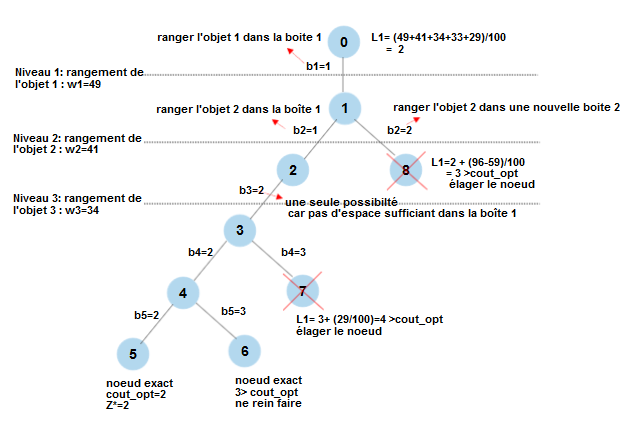
\includegraphics[width=\linewidth]{../figures/diag2.png}
\end{figure}
\section{Branch and bound amélioré}
Une version améliorée de l’algorithme Branch and Bound présenté ci-dessus. L’amélioration s’est faite en 2 étapes: 
\begin{enumerate}
    \item Utilisation de l’heuristique WFD (Worst Fit Decreasing) pour initialiser la solution optimale.
    \item Changement de la borne L1 utilisée par une autre borne plus puissante appelée L2. 
\end{enumerate}
\subsection*{Evaluation d'un noeud (Borne L2)}
Il a été prouvé que la borne L1 n’est efficace que quand les poids des objets sont petits, c’est à dire qu’on peut mettre plusieurs objets dans la même boîte. Si ce n’est pas le cas, et que les objets ont de grands poids ( proches de C) , cette borne n’aura aucun effet et l’algorithme fera une recherche exhaustive. 
C’est pour cela que la borne L2 à été proposée par Martello et Toth ,pour remédier à ce problème. 
on rappelle la formule de la borne L2, qui a été déjà présentée dans l’état de l’art:
\paragraph{rappel}
Soit \(\alpha\) un entier tels que :
\[0 \le \alpha \le C/2\]
On definie des classes d'articles suivantes: 
\[C_1 = \{a_i, \quad C-\alpha < v_i\} \]
\[C_2 = \{a_i, \quad C/2 < v_i \le C-\alpha\} \]
\[C_3 = \{a_i, \quad \alpha < v_i \le C/2\} \]
\(BI(I)\)  est donnée par la formule suivante:
\[BI(I)=max\{L(\alpha),\quad 0 \le \alpha \le C/2\}\]
Avec
\[L(\alpha)=|C_1|+|C_2|+max(0, \lceil{\frac{\sum_{j \in C_3}^{} v_j - (|C_2|*C - \sum_{j \in C_2}^{} v_j)\rceil }{C}})\]
\paragraph{Explication de la formule :}
Etant donnée que les objets des classes $C_1$ et $C_2$ ont un poids supérieur à $C/2$ chacun d'eux sera placé dans une boîte séparée pour le contenir, donc
$|C_1|+|C_2|$boîtes sont utilisées quelque soit la solution. De plus,aucun objet de l’ensemble $C_3$ ne peut être rangé dans une boîte contenant un objet de $C_1$ ( à cause de la contrainte de capacité). La capacité résiduelle (espace libre) des
$|C_2|$ boîtes est de : $C^*=|C_2|*c-\sum_{j \in C_2}^{} w_j$
Donc dans le meilleur des cas, cette capacité résiduelle va être remplie par les objets de $C_3$, et dans ce cas le nombre de nouvelles boîtes qu’on doit ouvrir est de :  
$\frac{\sum_{j \in C_3 -C^*}^{} w_j}{c}$ ( cette dernière formule utilise le même principe que la borne L1).
\subsection{Pseudocode}
%\begin{algorithm}
%   \caption{Branch and bound amélioré }   
%\end{algorithm}
\section{Recherche exhaustive }
Dans cette 3ème solution, on a implémenté une recherche exhaustive, qui consiste à parcourir l’ensemble des nœuds et leurs fils, sans aucun élagage de nœuds. Donc on aura le même algorithme que celui du branch and bound, en supprimant l’étape de l’évaluation du nœud pour décider de son élagage.  



\end{document}